\section{HRP-2Kai humanoid robot}
	\label{sec:hrp2kai}
	
	HRP-2Kai stands for Humanoid Robotics Platform no.~2 Improved (Kai means improvement in Japanese).
	This humanoid was developed in phase two of the Japanese national project HRP
	(Humanoid Robotics Project) and was recently improved to be able to cope with disaster response
	tasks~\cite{Kaneko}.
	
	This robot, depicted in \figurename~\ref{fig:HRP2Kai-robot}, has the kinematic structure shown
	in \figurename~\ref{fig:HRP2Kai-structure}.
	As seen in this diagram, the robot has 32 degrees of freedom (dof):
	6 at each leg, 2 at the waist, two at the head, 7 at each arm and 1 at each hand.
	This robot features a set of exteroceptive sensors that are actively used during the manipulation
	tasks: a 3D scanner system built in its head and four cameras, placed at the head, at the back and
	at each hand.
	The 3D scanner system was implemented with a Laser Range Finder (LRF) synchronized with the head
	pitch joint, as shown in \figurename~\ref{fig:3DScanner}.
	The hand camera is mounted in each hand as shown in \figurename~\ref{fig:Hand}, together with a
	LED light and a laser.
	It is worth to mention that this camera is not lined up with the longitudinal axis at the center
	of the hand.
	
	\begin{figure}[t]
		\begin{center}
			\subfloat[Actual robot.]{\label{fig:HRP2Kai-robot}
				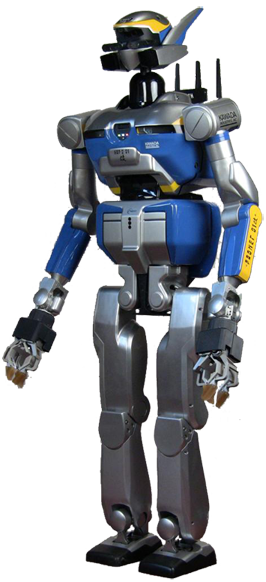
\includegraphics[height = 4.3cm]{img/HRP2Kai-robot}}
			\hspace{1cm}
			\subfloat[Structure.]{\label{fig:HRP2Kai-structure}
				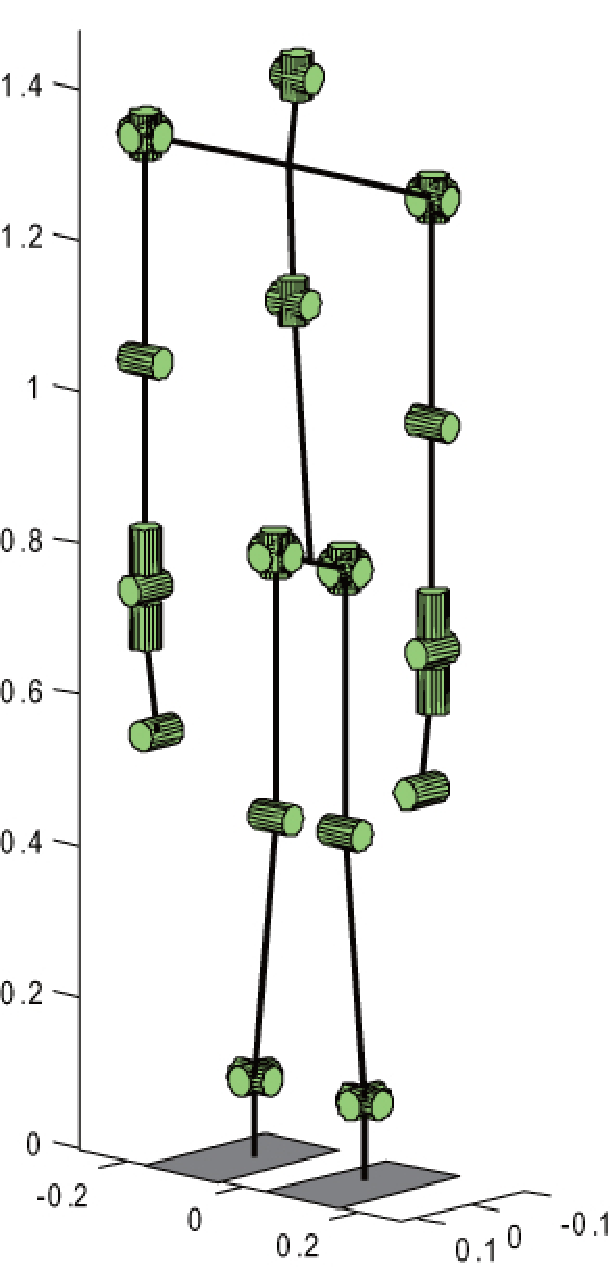
\includegraphics[height = 4.3cm]{img/HRP2Kai-structure}}
		\end{center}
		\caption{HRP-2 Kai humanoid robot.}
		\label{fig:HRP2Kai}
	\end{figure}
	
	\begin{figure}[b]
		\begin{center}
			\subfloat[3D scanner and head camera.]{\label{fig:3DScanner}
				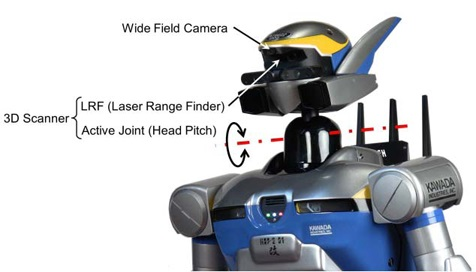
\includegraphics[height = 3cm]{img/3DScanner}}
			\hspace{0.25cm}
			\subfloat[Left hand camera.]{\label{fig:Hand}
				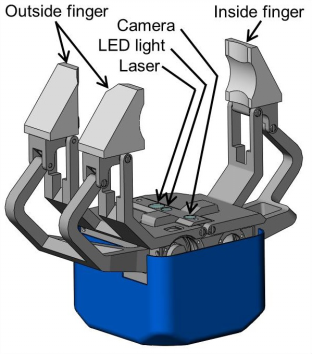
\includegraphics[height = 3cm]{img/Hand}}
		\end{center}
		\caption{Exteroceptive sensors of HRP-2 Kai~\cite{Kaneko}.}
		\label{fig:HRP2Kai}
	\end{figure}